\section{Aufbau}
    Im Folgenden wird der Aufbau des Algorithmus näher beschrieben.
    Nach einem kurzem Überblick werden die einzelnen Subsysteme detailliert erklärt.
    \subsection{Grundlegende Struktur}
    % oberflächliche Beschreibung des systems

    Es soll eine Liste an Layern, anhand der zuvor definierten Ziele, generiert werden.
    Die oberflächliche Struktur, des Generators, ist im unteren Flussdiagramm dargestellt.
    Für eine gegebene Anzahl an Layern in einer Rota wird für jedes Layer folgende Routine ausgeführt:

    \begin{itemize}
        \item wähle einen Modus, gewichtet nach den Mode-Wahrscheinlichkeiten $w_g$ und dem Mode-Spacing $\Delta_g$
        \item für den gewählten Modus werden die validen Maps gefiltert
        \begin{itemize}
            \item zunächst wird geprüft, welche Map im Modus repräsentiert ist
            \item aus den vorhanden Maps wird nach dem Distanz-Vote-Weight $w_m$ gewichtet eine Map gezogen
        \end{itemize}
        \item für die gezogene Map wird gewichtet nach dem Layerweight $w_l$ ein Layer gezogen
        \item die gezogenen Maps verbleiben für eine feste Maplänge im Memory-Kernel und sind damit für die nächsten Map Ziehungen nicht verfügbar
    \end{itemize}
    Im Folgenden werden die drei verschiedenen Schritte genauer erklärt und die verwendeten Weights definiert.
    \begin{figure}[htbp]
        \centering
        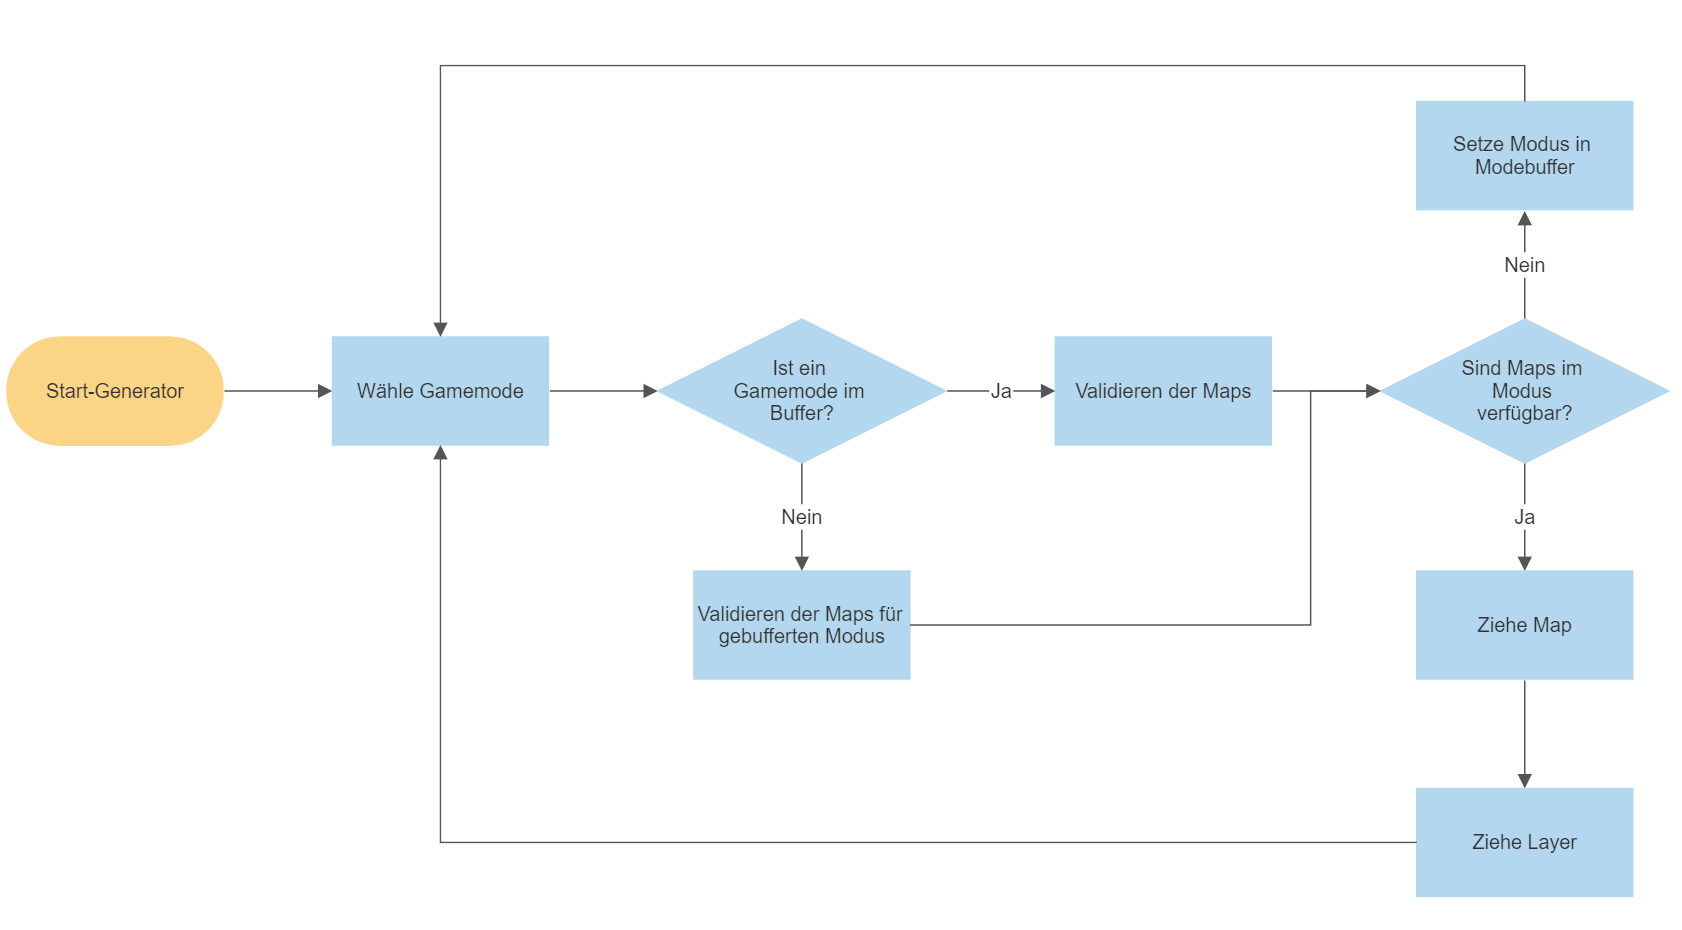
\includegraphics[width=0.8\textwidth]{FlowChartSuperficial.png}
        \caption{Oberflächlicher Ablauf des Generators.}
    \end{figure}

    \subsection{Aufbau im Detail - Mode}
        Wie zuvor erwähnt gibt es zwei Faktoren, welche die Ziehung des Modus beeinflussen:
        \begin{itemize}
            \item [1.] die Modeweights die zuvor gesetzt wurden $w_g$
            \item [2.] das Modespacing $\Delta_g$
        \end{itemize}
        Des Weiteren erlaubt der Generator eine Gruppierung der Modes in sogenannte \glqq{}Pools\grqq{}.
        Es gibt immer einen sogenannten \textit{main}-Pool.
        Ohne weitere Einstellungen ist jeder Modus, der gespielt werden soll, automatisch im Main-Pool enthalten.
        Neben diesem können noch weitere Pools definiert werden.
        In der momentanen Fassung existieren drei Pools:
        \begin{itemize}
            \item \textbf{main}: Der zuvor erwähnte Standard-Pool, beinhaltet \textit{RAAS} und \textit{AAS}
            \item \textbf{intermediates}: Beinhaltet die Modi \textit{Invasion} und \textit{TC}
            \item \textbf{reste}: Beinhaltet \textit{Destruction} und \textit{Insurgency}
        \end{itemize}

        Das \textbf{Modespacing} $\Delta_g\in{0,...,N}$ ist eine Zahl größer $0$ und maximal die Anzahl der Layer in einer Rota.
        Es sorgt nun dafür, dass für eine gegebene Anzahl an Runden nur der Main-Pool gezogen werden darf, wodurch eine \glqq{}Mindestzeit\grqq{} zwischen z.b. zwei Invasion Layern garantiert wird.
        Sollte die Zeitspanne seit dem letzten nicht-main Modus größer sein als das Modespacing, so wird mit den Pool und Mode-weights gewichtet ein Gamemode gewählt.
        Hierbei wird erst der Pool ausgewählt und anschließend im Pool der Modus.
        Es ist zu beachten, dass dies dazu führen kann und wird, dass nicht direkt nach Ablauf des Modespacings ein andere Pool drankommen muss.
        Das Design wurde mit Absicht so gewählt, um repetitive Modes zu verhindern.

        Das Modeweight $w_g$ setzt sich damit zusammen aus der Wahrscheinlichkeit den enthaltenen Pool zu ziehen und den Modus
        \begin{equation}
            w_g = \mathbb{P}(G=g|P=p) = \mathbb{P}(G=g)\mathbb{P}(P=p)
        \end{equation}
        wobei hier $G$ und $P$ die Zufallsvariablen \glqq{}Gamemode\grqq{} und \glqq{}Pool\grqq{} darstellen sollen.
        Durch das Modespacing ist die Wahrscheinlichkeit einen Modus zu ziehen ungleich größer als $w_g$.
        Dies muss bei der Wahl der Mode und Pool Wahrscheinlichkeiten beachtet werden.
        % \begin{equation}
        %     \label{eq:Modeweight}
        %     \mathbb{P}(G=g) = \frac{1}{N}\sum_{j=0}^{k_0}j\binom{N-j \Delta_g}{j}w_g^j(1-w_g)^{N-j(\Delta_g+1)}
        % \end{equation}
        % mit $w_g$ das oben definierte Weight, $N$ die Anzahl gezogener Layer und $k_0=\lfloor\frac{N}{N_0}\rfloor$ die maximale Anzahl an Zügen des Modus.
        % Der interessierte Leser vermag eine Herleitung im Anhang zu finden.

        Anschließend wird geprüft ob die Verfügbaren Maps den gewählten Modus enthalten. Sollte dies nicht der Fall sein so wird der Modus in einem Buffer gespeichert und es wird erneute ein Modus zufällig gewählt.
        Der Buffer wird bei der nächsten Gelgenheit abgearbeitet.
    \subsection{Aufbau im Detail - Map}
    \label{sub:AufbauImDetail-Map}
        Für das ziehen der Maps werden Mapweights verwendet welche im wesentlichen von den Layervotes und der \glqq{}Ähnlichkeit\grqq{} der gespielten Maps abhängen.
        Zudem wird noch ein Memory Kernel verwendet der sich die letzten $k\geq 0$ gespielten Maps merkt um damit ungewollte Mapwiederholungen zu vermeiden.

        Das Weight errechnet sich als Produkt aus einem \glqq{}Distanz-Weight\grqq{} und einem \glqq{}Mapvote-Weight\grqq{}.
        \begin{equation}
            w_m(m,d,v) = \frac{1}{\mathcal{N}}w_d(d,m)w_v(v,m)
        \end{equation}
        mit $d$ der Distanz zur zuletzt gezogenen Map, $m$ der gewählten Map und $v$ die Summe aller Layervotes der Map im entsprechnden zuvor gewählten Modus.
        $\mathcal{N}$ ist die Norm des weights sodass $\sum_m w_m = 1$.
        \subsubsection{Map Charakteristiken}
            Um die verschiedenen Maps voneinander zu unterscheiden wird versucht bestimmende Charakteristiken der einzelnen Maps.
            Das heißt es werden bestimmte Eigenschaften der Map bewertet um diese untereinander zu vergleichen.
            Zum Beispiel kann man das \glqq{}Setting\grqq{} bewerten wie \glqq{}Wüste\grqq{} oder \glqq{}Schnee\grqq{} und damit verhindern das zu oft Wüstenmaps hintereinander gespielt werden.
            Die Idee ist eine Metrik $d(m_1,m_2)$ einzuführen welche einen \glqq{}Abstand\grqq{} zwischen zwei Maps $m_1$ und $m_2$ über die Map Charakteristiken misst.
            Zurzeit werden folgende Eigenschaften bewertet:
            \begin{table}[h]
                \centering
                \begin{tabular}{|| c ||}
                    \hline
                    \textbf{Mapcharakteristik}  \\
                    \hline
                    \hline
                    Mapgröße \\
                    \hline
                    Wald \\
                    \hline
                    Schnee \\
                    \hline
                    Wasser \\
                    \hline
                    Wüste \\
                    \hline
                    Grasland \\
                    \hline
                    Stadt \\
                    \hline
                    Berge \\
                    \hline
                    Felder \\
                    \hline
                \end{tabular}
                \caption{Benutzte Mapcharakteristiken.}
                \label{t:Aufbau:Charakteristiken}
            \end{table}
            Für jeder Map wird jeder Eigenschaft ein Wert zwischen $0$ und $1$ zugewiesen, wobei ersteres dafür steht, dass die Eigenschaft von der Map gar nicht erfüllt wird und letzteres bedeutet dass die Map diese Eigenschaft voll erfüllt.
            Die Einträge werden dann in einen Vektor $\vec{b}=(b_1,...,b_N)^T$ der aus den $N$ werten besteht zugeordnet und dieser wird Anschließend normiert sodass $|\vec{b}|=1$.
            Damit lässt sich jede Map als Punkt auf einem Teilstück einer $N$-Dimensionalen Kugel beschreiben.
            Dadurch kann man eine Distanz zwischen zwei Punkten auf besagtem Flächenstück definieren, welche gegeben ist durch
            \begin{equation}
                d(m_1, m_2) = 2\text{arccos}(\vec{b}_1\cdot\vec{b}_2),
            \end{equation}
            wobei $\vec{b}_1$ die Mapcharakteristiken der Map $m_1$ beschreibt und $\cdot$ das Standardskalarprodukt ist.
            Damit ist die Distanz zwischen zwei Maps rein durch den Winkel der beiden Vektoren gegeben.
            \begin{figure}[htbp]
                \centering
                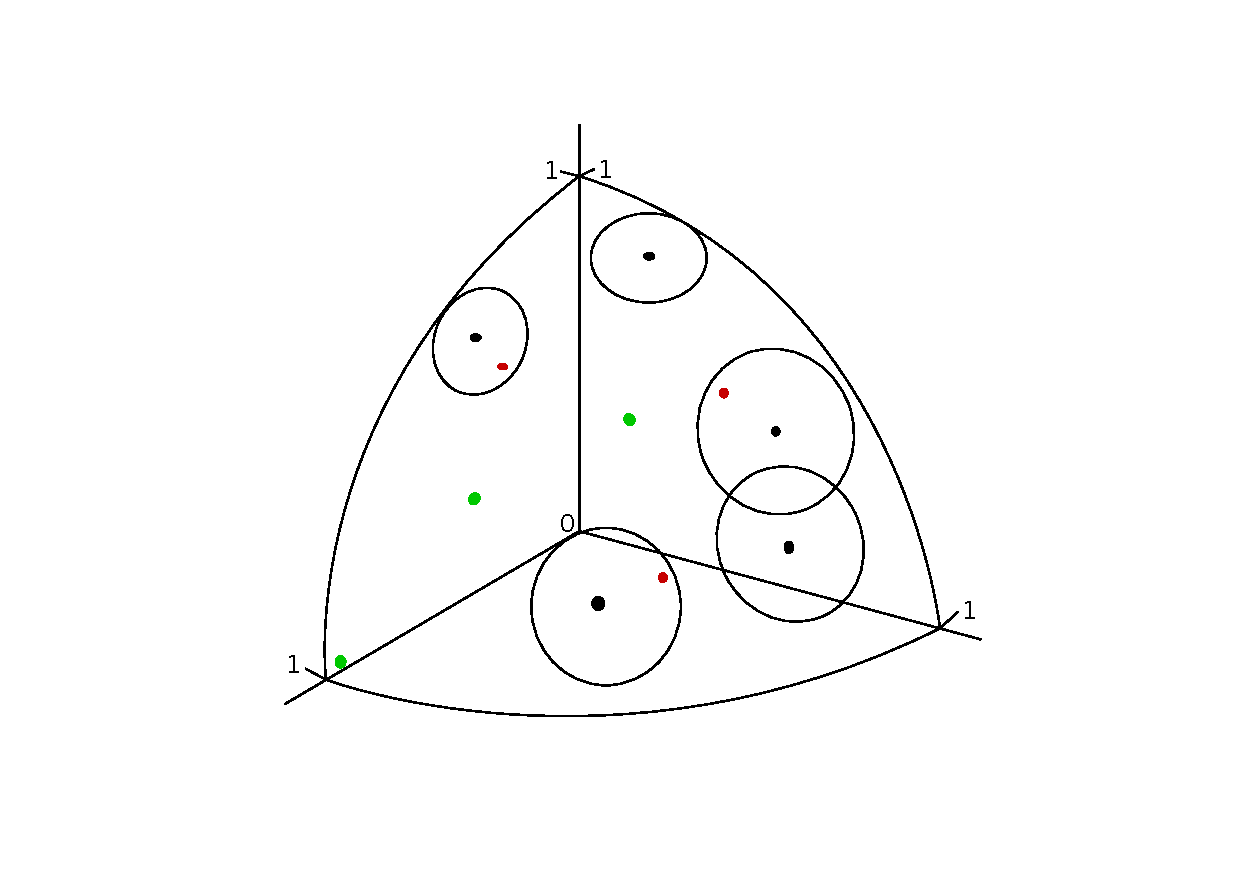
\includegraphics[width=0.8\textwidth]{Kugel.pdf}
                \caption{Skizze Kugeloberfläche für drei verwendete Biome, die verwendeten Radien sind nicht in der Größenordnung die im Generator verwendet wird.
                            Die schwarzen Punkte sind Maps, die gezogen wurden und noch im Memory Kernel liegen.
                            Die grünen Punkte sind Maps, welche für die nächste Runde zur Verfügung stehen.
                            Die roten Punkte sind Maps, welche gesperrt wurden aufgrund der Nähe zu einer bereits gezogenen Maps.}
            \end{figure}
            Maps, die ähnlich sind, wie z.b. \glqq{}Logar\grqq{} und \glqq{}Sumari\grqq{}, liegen nahe beieinander sind aber weit entfernt von z.B. ''Yehorivka''.
        \subsubsection{Distanzweight}
            Das Distanzweight ist eine allgemeine stückweise stetige Funktion definiert durch
            \begin{equation}
                w_d : \mathbb{R}^+ \rightarrow \mathbb{R}^+, d \mapsto w_d(d),
            \end{equation}
            und der Nebenbedingung $w_d(d)\overset{d\rightarrow 0}{\longrightarrow}0$.
            In der momentanen Version ist die Funktion gegeben durch
            \begin{equation}
                w_d(d) = 1_{[0,d_\text{min}]}(d)
            \end{equation}
            mit $d_\text{min}\geq 0$ als Mindestdistanz.
            Sollte eine Map näher als $d_\text{min}$ an einer zuvor gezogenen Map liegen, ist das Distanzweight und damit das Mapweight $0$ und wird damit nicht gezogen.
        \subsubsection{Mapvoteweight}
            Das Mapvoteweight soll die Beliebtheit der Map repräsentieren.
            Es ist allerdings nicht die Mapwahrscheinlichkeit gemessen an den Votes sondern ein rein internes Weight.
            Dies kommt daher, dass die Wahrscheinlichkeit eine Map zu ziehen durch den Memory Kernel und das Distanzweight stark nicht-linear vom Mapvoteweight abhängt und damit keine 1-zu-1 Relation gegeben ist.
            Die internen Weights müssen so gewählt sein, dass die Mapwahrscheinlichkeit zu der vorhergesagten Mapwahrscheinlichkeit passt.
            Leider ist dieses Problem nichtmehr geschlossen analytisch lösbar und benötigt numerische Lösungsmethoden.
            Näheres dazu im \nameref{sub:optimizer} Kapitel.
            Durch die Cutoff-Funktionen, die als Distanzweight verwendet werden kann,
            kann das Mapvoteweight als Funktion der gewollten Mapwahrscheinlichkeiten und der Anzahl an \glqq{}Nachbarn\grqq{} einer Map definiert werden.
            Mit Nachbar einer Map, ist jede Map gemeint, die näher als $d_{min}$ an der Map liegt.
            \begin{equation}
                \label{eq:mapweight}
                w_v(v) = \sum_{i,j = 0}^2 a_{ij}x^i y^j
            \end{equation}
            wobei $x$ die Anzahl an verbundenen Maps ist und $y$ die Mapwahrscheinlichkeit errechnet aus den Layervotes.
            Die Koeffizienten $a_{ij}\in\mathbb{R}$ müssen vorerst numerisch bestimmt werden.
        \subsubsection{Berechnung der Mapwahrscheinlichkeit}
            Um die internen Mapweights zu bestimmen, muss die Beliebtheit einer Map anhand der Layervotes errechnet werden.
            Dies erfolgt in zwei Schritten, getrennt für jeden einzelnen Modus.
            \begin{itemize}
                \item \textbf{Gewichtetes Mittel der Layervotes}\\
                Hierbei wird ein Mapvote als mittleres Layervote errechnet.
                Dafür wird ein gewichtetes arithmetisches Mittel verwendet damit \glqq{}Ausreißer\grqq{} die Mapbeliebtheit nicht zu stark beeinflussen.
                Der Mapvote ist gegeben durch
                \begin{equation}
                    \bar{v}_m = \sum_{l=1}^{N_l} \bar{w}_l v_l
                \end{equation}
                wobei $N_l$ die Anzahl an Layern, $v_l$ der Layervote-Wert eines Layers $l$ ist und das weight definiert ist als
                \begin{equation}
                    \bar{w}_l = \frac{w_l}{\sum_l w_l}
                \end{equation}
                mit
                \begin{equation}
                    w_l = \exp\left(-\left(v_l-\mu\right)^2\right)
                \end{equation}
                und $\mu$ der ungewichtete Mittelwert.
                \item \textbf{Mapweight und Wahrscheinlichkeit}\\
                Um eine Wahrscheinlichkeit zu bekommen wird zunächst der mittlere Vote auf das Intervall $[0,1]$ abgebildet.
                Dies geschieht mittels einer Sigmoid Funktion, sodass
                \begin{equation}
                    S(w) = \frac{1}{1+\exp\left(-a(w+b)\right)}
                \end{equation}
                nun das Weight ist aus dem die Mapwahrscheinlichkeit errechnet wird welche nur von den Layervotes abhängen. $a$ und $b$ sind zwei freie Parameter welche die Steigung und den Offset beeinflussen.
                Die Funktion bildet große $w$ auf $1$ ab und kleine $w$ auf $0$.
                Werte die näher an der Null sind werden damit auf das Intervall zwischen den Randpunten abgebildet.
                Damit kann die Mapwahrscheinlichkeit durch die Votes kontinuierlich angepasst werden und eine Map \glqq{}verschwindet\grqq{} erst nach mehreren negativen Votes aus der Rotation.
                Die Wahrscheinlichkeit, dass eine Map gezogen werden soll, ist dann gegeben durch
                \begin{equation}
                    \mathbb{P}(M=m) = \frac{S(v_m)}{\sum_m S(v_m)}
                \end{equation}
                und wird vor generation einer Rotaion zunächst berechnet.
                Dies erzeugt eine Verteilungsfunktion der Maps an welche die internen Mapweights angepasst werden müssen, bzw die Koeffizienten $a_{ij}$ müssen passend gewählt werden.
            \end{itemize}
            \begin{figure}[htbp]
                \centering
                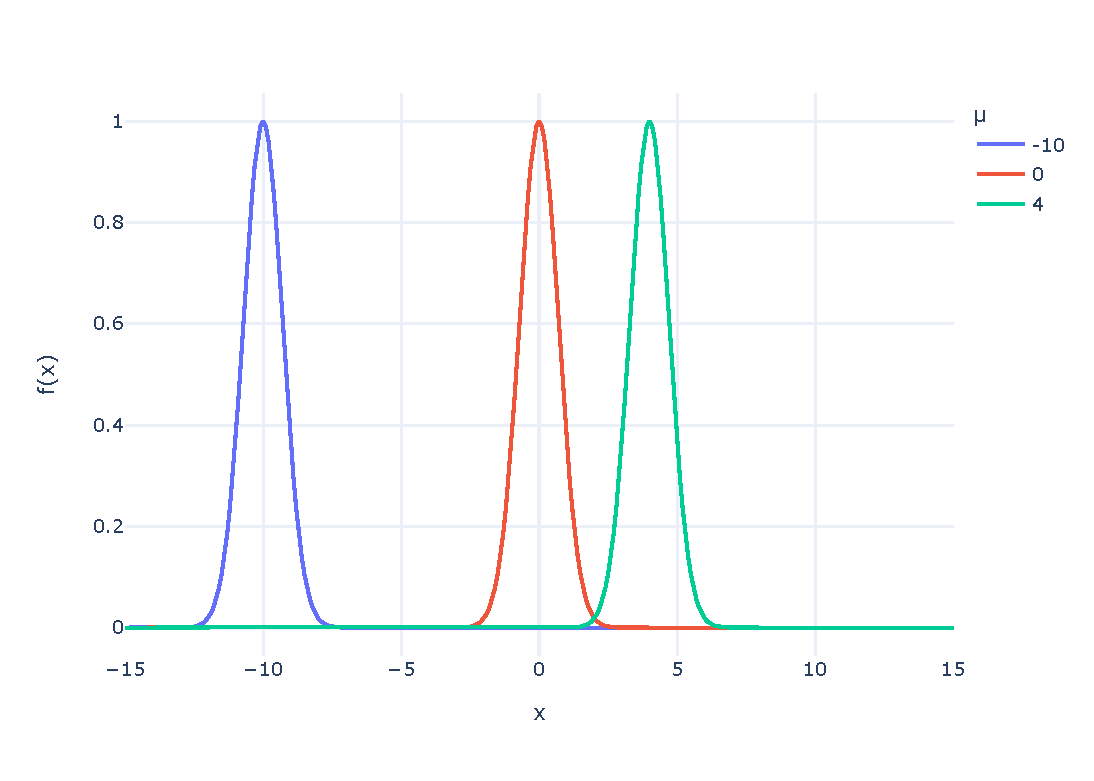
\includegraphics[width=0.8\textwidth]{plot_gaus.pdf}
                \caption{Die Weightfunktion $w_l(x)=f(x)$ für verschiedene Werte des ungewichteten Mittels $\mu$.
                        Je weiter weg ein Layervote $x$ vom Mittelwert liegt, desto kleiner ist das Weight und desto sträker wird dieses Layer damit bestraft. }
            \end{figure}
            \begin{figure}[htbp]
                \centering
                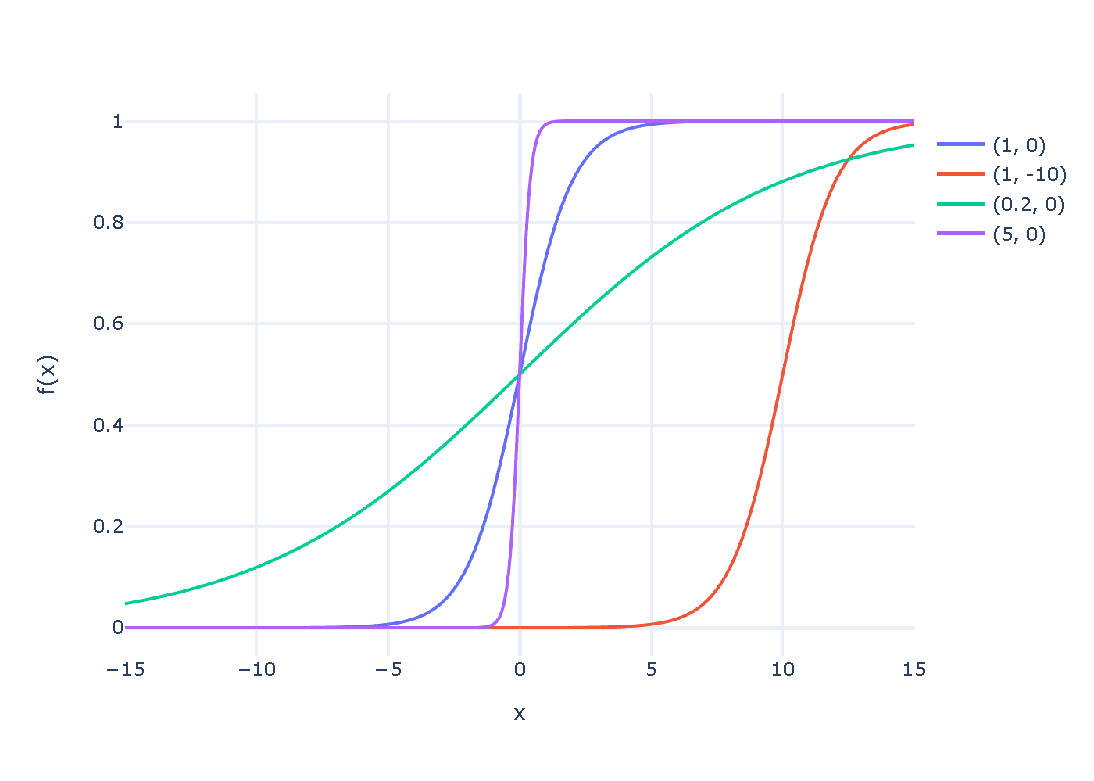
\includegraphics[width=0.85\textwidth]{plot_sigmoid.pdf}
                \caption{Die Sigmoidfunktion für mehrere Werte $a$ und $b$.
                            Für $b=0$ ist für alle Werte $a$ $f(0)=1/2$.
                            Der Parameter $b$ dient als Offset.}
            \end{figure}
        \subsubsection{Memory Kernel}
            Um das Wiederholen von Maps zu vermeiden wird ein Memory Kernel (\glqq{}Gedächtnis\grqq{}) verwendet.
            Das heißt, wenn ein Layer gezogen wurde, so wird die zum Layer zugeordnete Map in den Kernel gelegt.
            Das wird wiederholt, bis dieser mit einer Maximalen Anzahl an Maps gefüllt ist.
            Dies wird dadurch implementiert, dass das Mapweight effektiv $0$ ist für diese Map solange diese noch im Gedächtnis bleibt.
            Wenn nun in einem Modus eine Map gezogen wird, so darf diese nicht im Kernel liegen
        \subsubsection{Auswahl der Map}
            Nachdem nun alles notwendige definiert wurde wird kurz beschreiben wie eine Map gezogen wird.
            \begin{itemize}
                \item Nach Auswahl des Modus wird aus den vorhanden Maps zunächst das Distanzweight errechnet. Maps die zu Nahe an einer im Memory Kernel liegenden Map liegen können danach nichtmehr gezogen werden
                \item Aus den übrigen Maps wird gewichtet nach dem Mapweight eine Map gezogen
                \item Die ausgewählte Map wird in den Memory Kernel geschoben und sollte dieser voll sein, wird die älteste Map entfernt, wodurch ehemals gesperrte Maps wieder frei werden
            \end{itemize}
    \subsection{Aufbau im Detail - Layer}
    Sobald eine Map ausgewählt wurde, wird das Layer gewichtet nach dem Layerweights $w_l$ gezogen.
    Diese hängen nur von den Layervotes ab, welche mit der vorher genannten Sigmoidfunktion moduliert werden.
    Damit ist dann für $N_l$ Layer einer Map
    \todo{fix mathe}
    \begin{equation}
        w_l(j) = \frac{1}{\sum_{m=0}^{N_l}\frac{1}{\sum_{m=0}^{N_l}\left[1+\exp\left(-a(v_m+b)\right)\right]}}\frac{1}{1+\exp\left(-a(v_j+b)\right)}
    \end{equation}
    mit $v_j$ die Mapvote-Zahl des Layers $j$ der gegebenen Map.
    % \begin{figure}[htbp]
    %     \begin{tikzpicture}
    %         [scale=.8,auto=left,every node/.style={circle,fill=blue!20}]
    %         \node (n1) at (1,10) {Gorodok};
    %         \node (n2) at (4,8)  {Yehorivka};
    %         \node (n3) at (8,9)  {Blackcoast};
    %         \node (n4) at (11,8) {Skorpo};
    %         \node (n5) at (15,10) {Sumari};
    %         \node (n6) at (20,8)  {Logar};
    %         \node (n7) at (17,9)  {Fallujah};
    %         \foreach \from/\to in {n1/n2,n1/n3,n2/n3,n3/n4,n5/n6,n5/n7,n6/n7}
    %         \draw (\from) -- (\to);
    %     \end{tikzpicture}
    % \caption{Cluster}
    % \end{figure}